\documentclass[greek]{beamer}
%\usepackage{fontspec}
\usepackage{amsmath,amsthm}
\usepackage{unicode-math}
\usepackage{xltxtra}
\usepackage{graphicx}
\usetheme{CambridgeUS}
\usecolortheme{seagull}
\usepackage{hyperref}
\usepackage{ulem}
\usepackage{xgreek}

\usepackage{pgfpages}
\usepackage{tikz}
\usepackage{tkz-tab}
%\setbeameroption{show notes on second screen}
%\setbeameroption{show only notes}

\setsansfont{Noto Serif}

\usepackage{multicol}

\usepackage{appendixnumberbeamer}

\setbeamercovered{transparent}
\beamertemplatenavigationsymbolsempty

\title{Συναρτήσεις}
\subtitle{Μονοτονία}
\author[Λόλας]{Κωνσταντίνος Λόλας}
\date{}

\begin{document}

\begin{frame}
  \titlepage
\end{frame}

\section{Θεωρία}
\begin{frame}{Κάτι που αφήσαμε πιο πριν...}
  Δεν μπορούσαμε να υπολογίσουμε όλων των συναρτήσεων την μονοτονία π.χ.
  \begin{enumerate}
    \item $e^x-x$
    \item $x^3-2x+1$
    \item $\ln x - x^2$
  \end{enumerate}
\end{frame}

\begin{frame}{Spoiler}
  Σε τι βοηθάει η κλίση και ασχολούμαστε? (δικό σας!)
  \begin{itemize}
    \item<2-> Προσέγγιση συνάρτησης
      \begin{itemize}
        \item<3-> Για υπολογισμούς κοντά στο $x_0$, π.χ. $\sqrt{4,05}$
        \item<4-> Για να ξέρουμε αν θα μειώσει ή θα αυξηθεί κοντά στο $x_0$
        \item<5-> Για υπολογισμό εμβαδού κάτω από την γραφική
      \end{itemize}
    \item<6-> Εύρεση ριζών
    \item<7-> Φυσική (ρυθμός μεταβολής)
  \end{itemize}
\end{frame}

\begin{frame}[label=Θεώρημα1]{Μονοτονία}
  \begin{block}{Μονοτονία}
    Έστω μία συνάρτηση $f$ συνεχής στο $Δ$. Αν $f'(x)>0$ σε κάθε εσωτερικό σημείο $x$ του $Δ$, τότε η $f$ είναι γνησίως αύξουσα στο $Δ$
  \end{block}
  \onslide<2-> Όμοια για $f'(x)<0$

  \hyperlink{Απόδειξη1}{\beamerbutton{Απόδειξη}}
\end{frame}

\begin{frame}{Από εδώ και εμπρός...}
  \begin{enumerate}
    \item<1-> Ξαναλύνουμε όλες τις ασκήσεις με μονοτονία, τώρα όμως ΟΛΕΣ
    \item<2-> Όσοι δεν τα μάθανε καλά, είναι ευκαιρία τώρα να επιστρέψουν
    \item<3-> Όσοι τα είχατε καταλάβει ευκαιρία για επανάληψη
    \item<4-> Θα ασχολούμαστε με πρόσημα!!!!
  \end{enumerate}
\end{frame}

\begin{frame}{Και λίγο κατανόηση δεν βλάπτει}
  \begin{enumerate}
    \item<1-> Αν $f'>0$ τότε $f\uparrow$ \only<2> {\emph{ΛΑΘΟΣ!!!!!!!!!!}}
    \item<3-> Αν $f\uparrow$ τότε $f'>0$ \only<4> {\emph{ΛΑΘΟΣ!!!!!!!!!!}}
    \item<5-> Αν $f\uparrow$ τότε $f'\ge 0$ \only<6> {\emph{ΛΑΘΟΣ!!!!!!!!!!}}
    \item<7-> Αν $f'\ne 0$ τότε $f$ γνησίως μονότονη \only<8> {\emph{ΛΑΘΟΣ!!!!!!!!!!}}
  \end{enumerate}
\end{frame}

\section{Ασκήσεις}
\subsection{Άσκηση 1}
\begin{frame}[label=Άσκηση1]{Εξάσκηση 1}
  Να μελετήσετε τις παρακάτω συναρτήσεις ως προς τη μονοτονία
  \begin{enumerate}
    \item<1-> $f(x)=e^x+x-1$
    \item<2-> $f(x)=x^3-x^2+x-1$
    \item<3-> $f(x)=ημx-2x$
    \item<4-> $f(x)=(x-1)^3-2$
    \item<5-> $f(x)=x-ημx-1$
  \end{enumerate}

  % \hyperlink{Λύση1}{\beamerbutton{Λύση}}
\end{frame}

\subsection{Άσκηση 2}
\begin{frame}[label=Άσκηση2]{Εξάσκηση 2}
  Να βρείτε τα διαστήματα μονοτονίας των συναρτήσεων
  \begin{enumerate}
    \item<1-> $f(x)=x^2-2x-3$
    \item<2-> $f(x)=\dfrac{x^3}{3}+\dfrac{x^2}{2}-2x-1$
    \item<3-> $f(x)=\dfrac{1}{4}x^4-x-1$
    \item<4-> $f(x)=\dfrac{x^4}{4}-\dfrac{7}{2}x^2+6x-1$
    \item<5-> $f(x)=3x^4-4x^3-1$
  \end{enumerate}

  % \hyperlink{Λύση2}{\beamerbutton{Λύση}}
\end{frame}

\subsection{Άσκηση 3}
\begin{frame}[label=Άσκηση3]{Εξάσκηση 3}
  Να βρείτε τα διαστήματα μονοτονίας των συναρτήσεων
  \begin{enumerate}
    \item<1-> $f(x)=x-\ln (x^2+1)$
    \item<2-> $f(x)=\dfrac{x^2-x+1}{x-1}$
    \item<3-> $f(x)=\ln |x|+\dfrac{1}{2x^2}$
  \end{enumerate}

  % \hyperlink{Λύση3}{\beamerbutton{Λύση}}
\end{frame}

\subsection{Άσκηση 4}
\begin{frame}[label=Άσκηση4]{Εξάσκηση 4}
  Να βρείτε τα διαστήματα μονοτονίας των συναρτήσεων
  \begin{enumerate}
    \item<1-> $f(x)=\sqrt{x^2+1}$
    \item<2-> $f(x)=x-2\sqrt{x}$
    \item<3-> $f(x)=x\sqrt{x+1}$
  \end{enumerate}

  % \hyperlink{Λύση4}{\beamerbutton{Λύση}}
\end{frame}

\subsection{Άσκηση 5}
\begin{frame}[label=Άσκηση5]{Εξάσκηση 5}
  Να βρείτε τα διαστήματα μονοτονίας των συναρτήσεων
  \begin{enumerate}
    \item<1-> $f(x)=2e^x-x+1$
    \item<2-> $f(x)=x^x$, $x>0$
    \item<3-> $f(x)=(x-2)e^x-\dfrac{x^2}{2}+x+1$
  \end{enumerate}

  % \hyperlink{Λύση5}{\beamerbutton{Λύση}}
\end{frame}

\subsection{Άσκηση 6}
\begin{frame}[label=Άσκηση6]{Εξάσκηση 6}
  Να βρείτε τα διαστήματα μονοτονίας των συναρτήσεων
  \begin{enumerate}
    \item<1-> $f(x)=x^2-xημx-συνx$
    \item<2-> $f(x)=\dfrac{1}{1+ημx}$, $x\in [0,\pi]$
    \item<3-> $f(x)=εφx-x$, $x\in \left( -\dfrac{\pi}{2},\dfrac{\pi}{2} \right) $
  \end{enumerate}

  % \hyperlink{Λύση6}{\beamerbutton{Λύση}}
\end{frame}

\subsection{Άσκηση 7}
\begin{frame}[label=Άσκηση7]{Εξάσκηση 7}
  Να μελετήσετε τις παρακάτω συναρτήσεις ως προς τη μονοτονία
  \begin{enumerate}
    \item<1-> $f(x)=\begin{cases}
          1-\ln (x^2+1) & ,x<0    \\
          e^x-x         & ,x\ge 0
        \end{cases}$
    \item<2-> $f(x)=\begin{cases}
          x^2-2x     & ,x<0    \\
          32x^3-3x^2 & ,x\ge 0
        \end{cases}$
  \end{enumerate}

  %\hyperlink{Λύση7}{\beamerbutton{Λύση}}
\end{frame}

\subsection{Άσκηση 8}
\begin{frame}[label=Άσκηση8]{Εξάσκηση 8}
  Έστω $f:[0,4]\to\mathbb{R}$ μία συνάρτηση η οποία είναι συνεχής και η γραφική παράσταση της $f'$ φαίνεται στο σχήμα. Να βρείτε τα διαστήματα μονοτονίας της $f$.

  \centering
  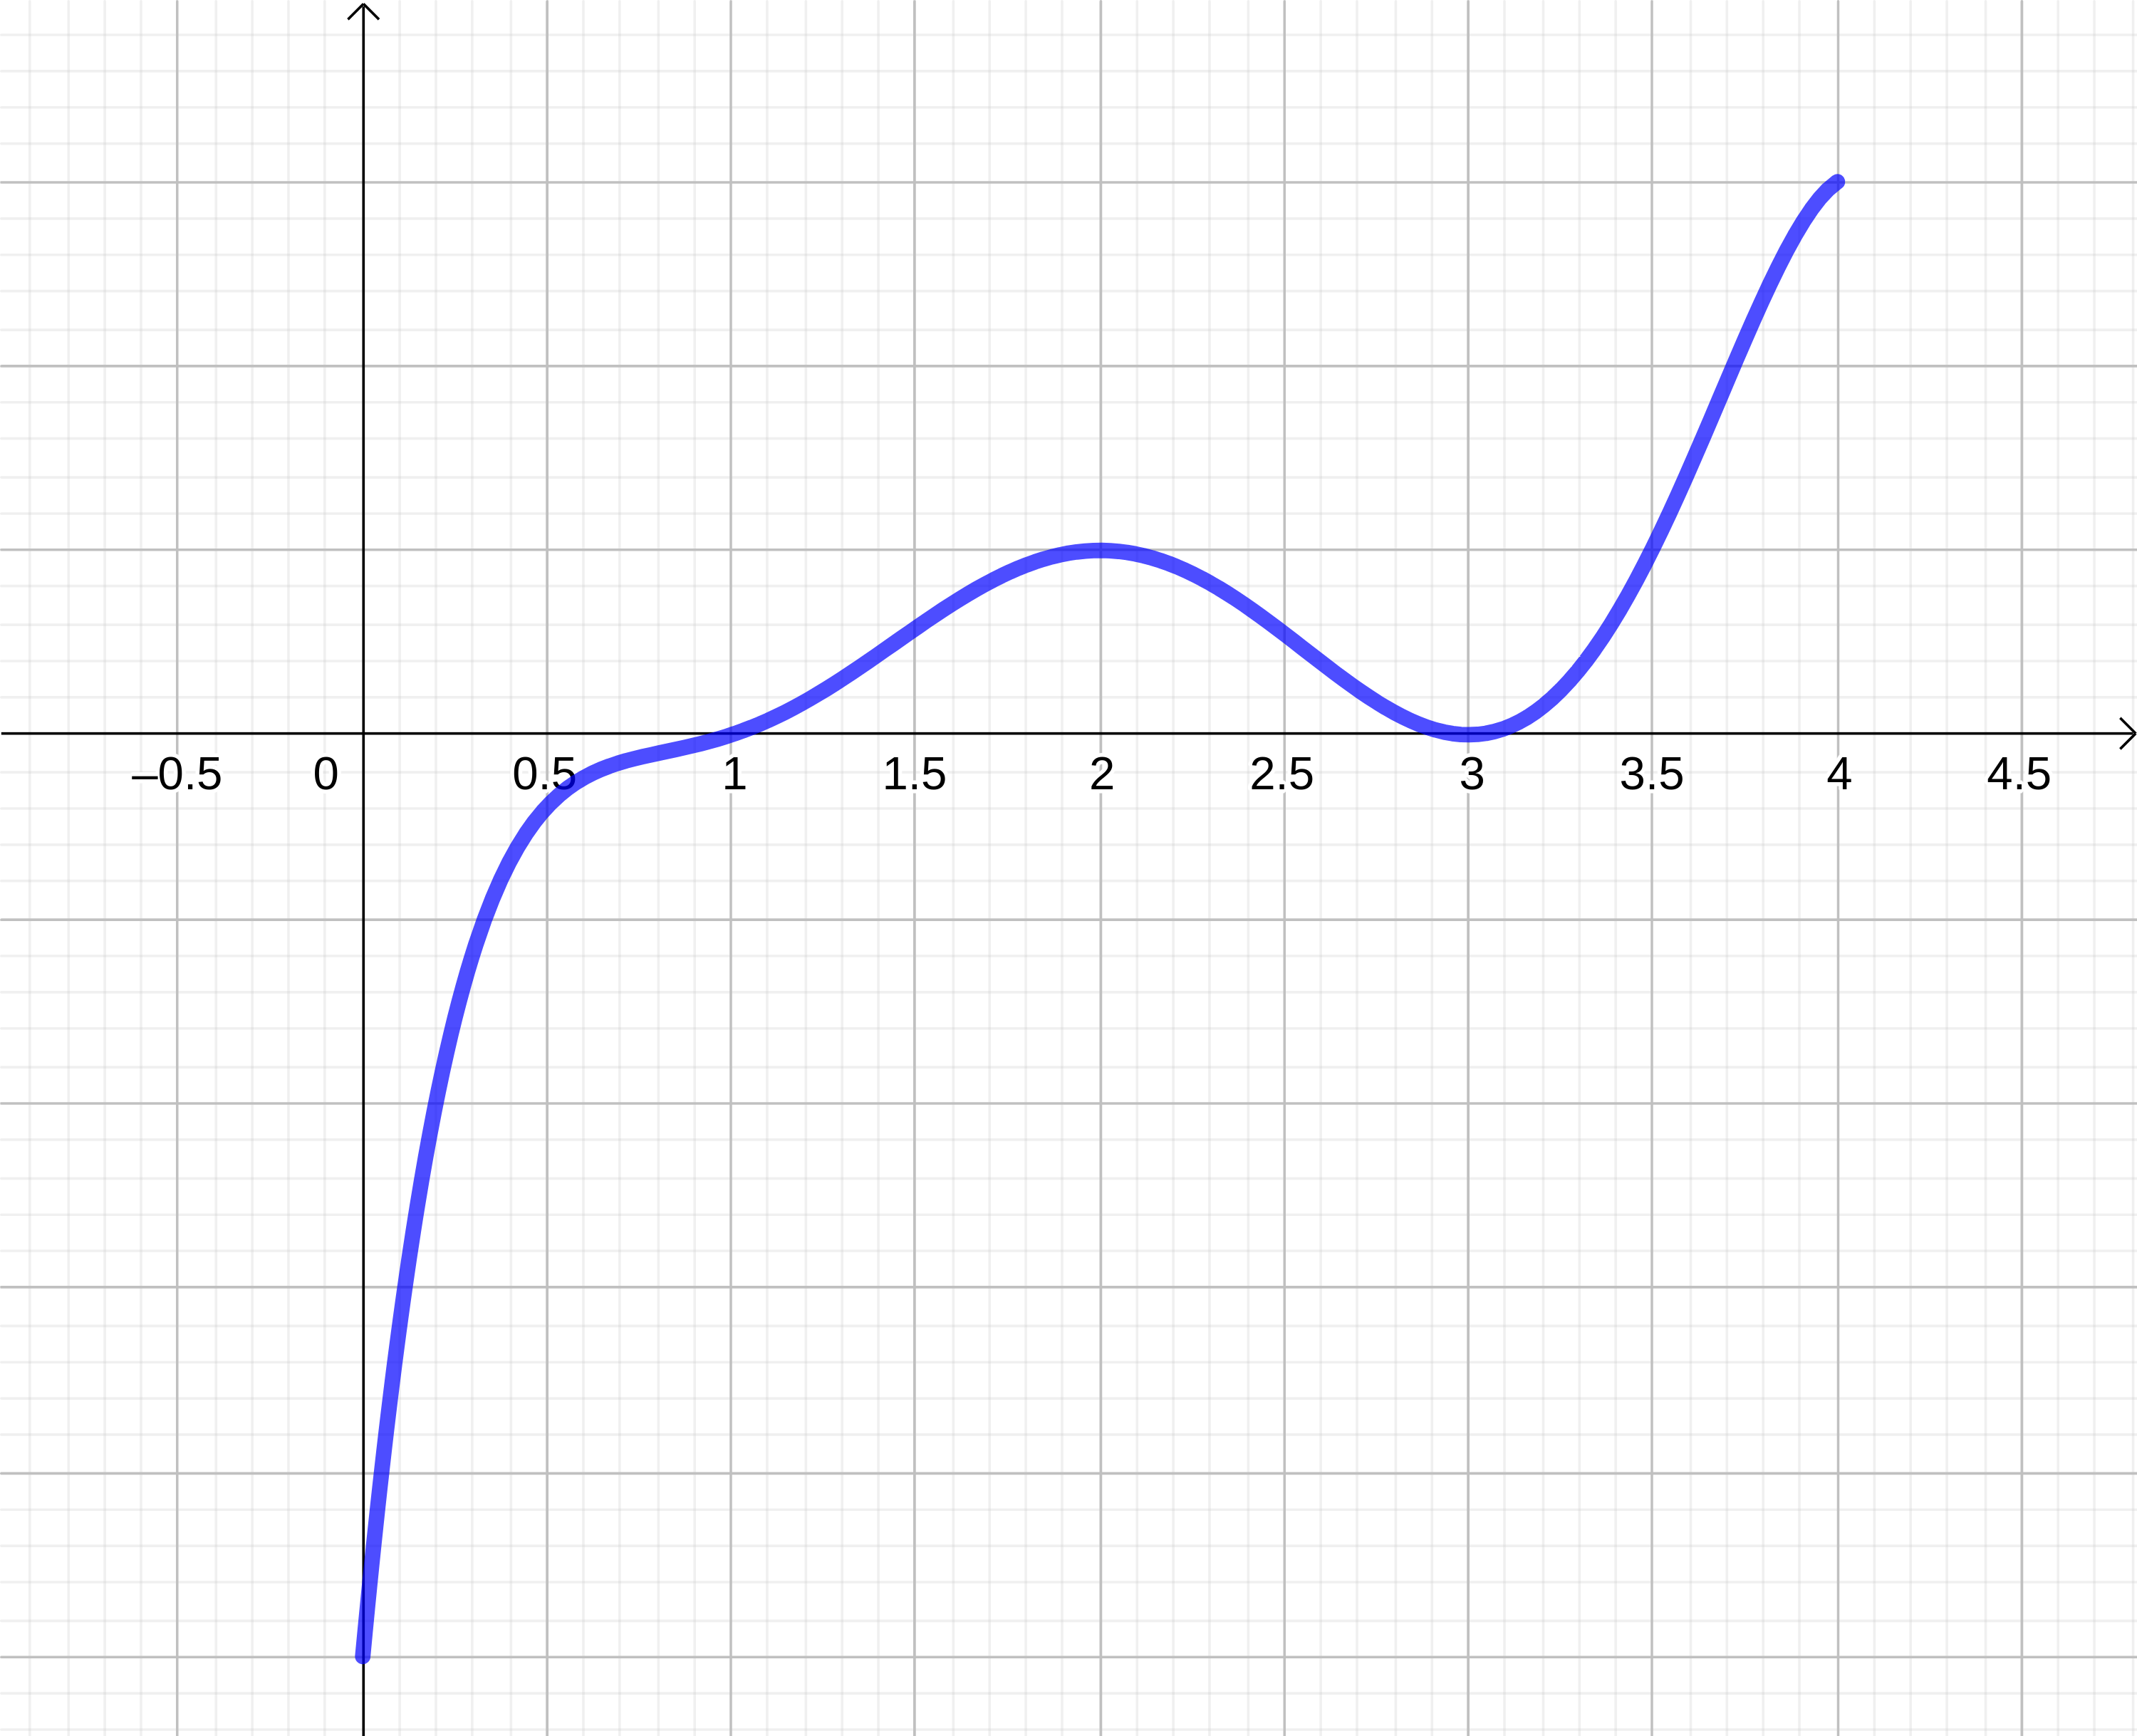
\includegraphics[width=0.6\textwidth]{"images/2.6.2 Μονοτονία.png"}

  %\hyperlink{Λύση8}{\beamerbutton{Λύση}}
\end{frame}

\subsection{Άσκηση 9}
\begin{frame}[label=Άσκηση9]{Εξάσκηση 9}
  Να βρείτε τις ρίζες και το πρόσημο της συνάρτησης $f(x)=e^x+2x-1$

  %\hyperlink{Λύση9}{\beamerbutton{Λύση}}
\end{frame}

\subsection{Άσκηση 10}
\begin{frame}[label=Άσκηση10]{Εξάσκηση 10}
  Να βρείτε τα διαστήματα μονοτονίας της συνάρτησης $f(x)=e^x-e\ln x$

  %\hyperlink{Λύση10}{\beamerbutton{Λύση}}
\end{frame}

\subsection{Άσκηση 11}
\begin{frame}[label=Άσκηση11]{Εξάσκηση 11}
  Να μελετήσετε τις παρακάτω συναρτήσεις ως προς τη μονοτονία
  \begin{enumerate}
    \item<1-> $f(x)=\ln x-\dfrac{\ln x}{x}$
    \item<2-> $f(x)=\begin{cases}
          \dfrac{ημx}{x} & ,x\in (0,\pi) \\
          1              & ,x=0
        \end{cases}$
  \end{enumerate}

  %\hyperlink{Λύση11}{\beamerbutton{Λύση}}
\end{frame}

\subsection{Άσκηση 12}
\begin{frame}[label=Άσκηση12]{Εξάσκηση 12}
  Να μελετήσετε τις παρακάτω συναρτήσεις ως προς τη μονοτονία
  \begin{enumerate}
    \item<1-> $f(x)=e^x-\dfrac{x^2}{2}-x-1$
    \item<2-> $f(x)=2x\ln x-x^2$
    \item<3-> $f(x)=e^{-x}+\ln x$
    \item<4-> $f(x)=-σφx+\dfrac{1}{x}$, $x\in (0,\pi)$
  \end{enumerate}

  %\hyperlink{Λύση12}{\beamerbutton{Λύση}}
\end{frame}

\subsection{Άσκηση 13}
\begin{frame}[label=Άσκηση13]{Εξάσκηση 13}
  Να βρείτε τα διαστήματα μονοτονίας των συναρτήσεων
  \begin{enumerate}
    \item<1-> $f(x)=-2συνx-x$, $x\in [0,\pi]$
    \item<2-> $f(x)=e^xσυνx$, $x\in \left[ 0,\pi \right) $
  \end{enumerate}

  %\hyperlink{Λύση13}{\beamerbutton{Λύση}}
\end{frame}

\subsection{Άσκηση 14}
\begin{frame}[label=Άσκηση14]{Εξάσκηση 14}
  Να βρείτε τα διαστήματα μονοτονίας των συναρτήσεων
  \begin{enumerate}
    \item<1-> $f(x)=2ημx+εφx-3x$, $x\in \left[ 0,\dfrac{\pi}{2} \right) $
    \item<2-> $f(x)=\dfrac{σφx}{x}$, $x\in (0,\pi) $
  \end{enumerate}

  %\hyperlink{Λύση14}{\beamerbutton{Λύση}}
\end{frame}

\subsection{Άσκηση 15}
\begin{frame}[label=Άσκηση15]{Εξάσκηση 15}
  Να βρείτε τα διαστήματα μονοτονίας των συναρτήσεων
  \begin{enumerate}
    \item<1-> $f(x)=x\sqrt{4-x^2}$
    \item<2-> $f(x)=x-\sqrt{x^2-1}$
    \item<3-> $f(x)=\dfrac{1}{2}x^2-2x^{\frac{3}{2}}+2x$
  \end{enumerate}

  %\hyperlink{Λύση15}{\beamerbutton{Λύση}}
\end{frame}

\subsection{Άσκηση 16}
\begin{frame}[label=Άσκηση16]{Εξάσκηση 16}
  Έστω $f:[1,+\infty)\to\mathbb{R}$ μία συνάρτηση η οποία είναι δύο φορές παραγωγίσιμη με $f(1)=f'(1)=0$ και ισχύει $f''(x)>0$ για κάθε $x>1$. Να αποδείξετε ότι η συνάρτηση $g(x)=\begin{cases}
      \dfrac{f(x)}{x-1} & ,x>1 \\
      0                 & ,x=1
    \end{cases}$, είναι γνησίως αύξουσα

  %\hyperlink{Λύση16}{\beamerbutton{Λύση}}
\end{frame}

\subsection{Άσκηση 17}
\begin{frame}[label=Άσκηση17]{Εξάσκηση 17}

  Έστω $f:[0,+\infty)\to\mathbb{R}$ μία συνάρτηση με $f(0)=0$ η οποία είναι παραγωγίσιμη με $f'(0)=0$ και η $f'$ είναι γνησίως αύξουσα. Να αποδείξετε ότι η συνάρτηση $g(x)=\begin{cases}
      \dfrac{f(x)}{x} & ,x>0 \\
      0               & ,x=0
    \end{cases}$, είναι γνησίως φθίνουσα

  %\hyperlink{Λύση17}{\beamerbutton{Λύση}}
\end{frame}

\subsection{Άσκηση 18}
\begin{frame}[label=Άσκηση18]{Εξάσκηση 18}
  Να βρείτε τις τιμές του $a\in \mathbb{R}^*$, για τις οποίες η συνάρτηση

  $$f(x)=\dfrac{ax^3}{3}+x^2+x-1$$

  είναι γνησίως αύξουσα

  %\hyperlink{Λύση18}{\beamerbutton{Λύση}}
\end{frame}

\subsection{Άσκηση 19}
\begin{frame}[label=Άσκηση19]{Εξάσκηση 19}
  Να αποδείξετε ότι η συνάρτηση $f(x)=\dfrac{2}{3}\sqrt{x^3}+συνx$ είναι γνησίως αύξουσα

  %\hyperlink{Λύση19}{\beamerbutton{Λύση}}
\end{frame}

\subsection{Άσκηση 20}
\begin{frame}[label=Άσκηση20]{Εξάσκηση 20}
  Να μελετήσετε ως προς τη μονοτονία τις συναρτήσεις
  \begin{enumerate}
    \item<1-> $f(x)=e^x-x+\ln (1+x^2)$
    \item<2-> $f(x)=\ln x+x+e^{-x}$
  \end{enumerate}

  %\hyperlink{Λύση20}{\beamerbutton{Λύση}}
\end{frame}


\appendix

\section{Αποδείξεις}
\begin{frame}[label=Απόδειξη1]{Απόδειξη μονοτονίας συνάρτησης}
  Θα δείξουμε ότι για κάθε $x_1<x_2\in Δ \implies f(x_1)<f(x_2)$.

  \onslide<1-> Στο $[x_1,x_2]$ είναι παραγωγίσιμη, άρα θα ισχύει το ΘΜΤ

  \onslide<2-> Υπάρχει $ξ\in Δ$ ώστε $f'(ξ)=\dfrac{f(x_2)-f(x_1)}{x_2-x_1}$.

  \onslide<3-> Αλλά $f'(x)>0$ για κάθε $x\in Δ$

  \onslide<4-> Άρα $f'(ξ)=\dfrac{f(x_2)-f(x_1)}{x_2-x_1}>0$

  \onslide<5-> $f(x_2)>f(x_1)$

  \hyperlink{Θεώρημα1}{\beamerbutton{Πίσω στη θεωρία}}
\end{frame}


% \section{Λύσεις Ασκήσεων}
% \begin{frame}
%  \tableofcontents
% \end{frame}
%
% \subsection{Άσκηση 1}
% \begin{frame}[label=Λύση1]
%  Με θεώρημα ενδιαμέσων τιμών. Η συνάρτηση είναι συνεχής στο $[10,11]$ με $f(10)=1024$ και $f(11)=2048$. Αφού $2023\in (1024,2048)$ υπάρχει $x_0$...
%
%  \hyperlink{Άσκηση1}{\beamerbutton{Πίσω στην άσκηση}}
% \end{frame}
%
% \subsection{Άσκηση 2}
% \begin{frame}[label=Λύση2]
%  Με Bolzano ή με μέγιστης ελάχιστης τιμής και ΘΕΤ.
%
%  \begin{gather*}
%   f(3)<f(2)<f(1) \\
%   3f(3)<f(1)+f(2)+f(3)<3f(1) \\
%   f(3)<\dfrac{f(1)+f(2)+f(3)}{3}<f(1)
%  \end{gather*}
%
%  \hyperlink{Άσκηση2}{\beamerbutton{Πίσω στην άσκηση}}
% \end{frame}
%
% \subsection{Άσκηση 3}
% \begin{frame}[label=Λύση3]
%  Προφανές ελάχιστο στα $x_1=1$ και $x_2=3$. Ως συνεχής στο $[1,3]$ έχει σίγουρα ΚΑΙ μέγιστο στο $(1,3)$
%
%  \hyperlink{Άσκηση3}{\beamerbutton{Πίσω στην άσκηση}}
% \end{frame}
%
% \subsection{Άσκηση 4}
% \begin{frame}[label=Λύση4]
%  Η συνάρτηση `απόστασης` $f(x)-x$ είναι ορισμένη στο κλειστό διάστημα και έχει σίγουρα μέγιστο
%
%  \hyperlink{Άσκηση4}{\beamerbutton{Πίσω στην άσκηση}}
% \end{frame}
%
% \subsection{Άσκηση 5}
% \begin{frame}[label=Λύση5]
%  Όμοια με την Άσκηση 2
%
%  \hyperlink{Άσκηση5}{\beamerbutton{Πίσω στην άσκηση}}
% \end{frame}
%
% \subsection{Άσκηση 6}
% \begin{frame}[label=Λύση6]
%  \begin{enumerate}
%   \item Είναι γνησίως αύξουσα άρα $(f(+\infty),f(-\infty))$
%   \item Προφανώς $[f(0),f(1)]$...
%  \end{enumerate}
%
%  \hyperlink{Άσκηση6}{\beamerbutton{Πίσω στην άσκηση}}
% \end{frame}

\end{document}
